\section{Perspectiva de continuidade do trabalho}

Na próxima fase do projeto, utilizaremos modelos estatísticos e de inteligencia artificial para séries temporais, para gerar as projeções dessas variáveis, não só para o Pará mas para as regiões intermediárias  a fim de identificar a tendencias desses produtos localmente. 

A intenção da coleta dos dados é voltada para utilização em modelos de aprendizado de máquina e predições baseadas em modelos estatísticos. Neste ínterim, o modelo ARIMA Hierárquico será a aposta inicial para a continuidade desse trabalho, pois se adapta bem a séries relativamente pequenas e possui boa adaptabilidade e acurácia já constatada em diversos trabalhos. 

A otimização ou tuning de modelos é o processo de procura por valores de configuração que buscam pelo conjunto de parâmetros que geram as melhores métricas para os modelos treinados \cite{thornton2013auto}. Deverão ser utilizados algoritmos de otimização a exemplo: RandomSearch e GridSearch na tentativa de encontrar parâmetros que otimizem o resultado gerado pelos modelos. O RandomSearch deverá ser utilizado como inicializador do processo de procura, já que explora o espaço de parâmetros de forma mais ampla e muito comumente encontrando um conjunto de valores paramétricos razoavelmente bons \cite{feurer2019hyperparameter}, enquanto GridSearch irá combinar todos os valores dentro de conjuntos definidos de configurações e retornará o conjunto de parâmetros com melhor performance.

A mensuração do desempenho do modelo em face a aplicação de técnicas de otimização deve ser através de validação cruzada, dado que a otimização pode implicar no overfitting ou underfitting de dados, dependendo do tamanho do conjunto utilizado \cite{feurer2019hyperparameter}. A validação cruzada consiste na separação dos dados em $n$ diferentes conjuntos e após isso, um dos conjuntos será utilizado como teste e os demais como treino \cite{scikit-learn}, isso acontecerá até todos os conjuntos tenham sido usados como teste. Após essa etapa, será possível obter uma distribuição de erros gerados pelo modelos em cada conjunto.

\begin{figure}[hbt!]
    \centering
    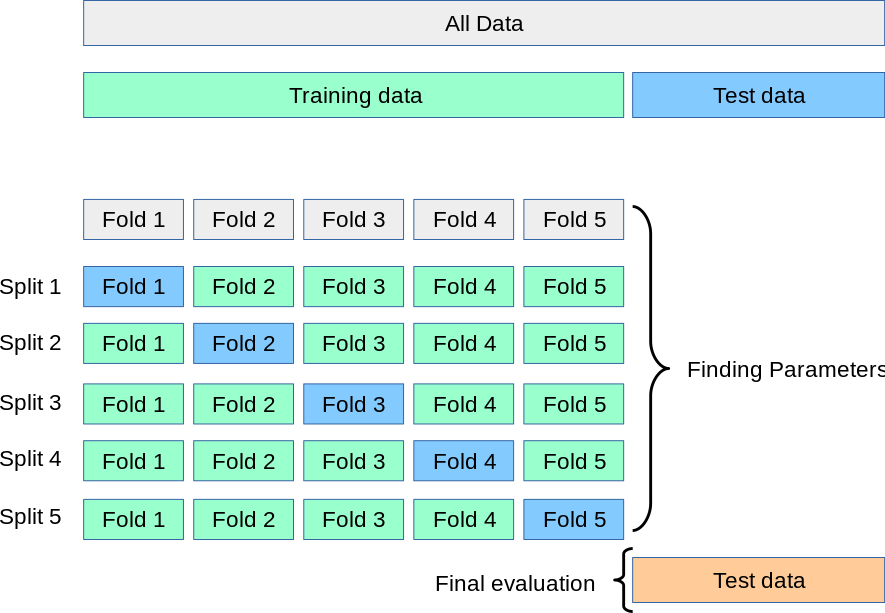
\includegraphics[width=0.8\columnwidth]{src/grid_search_cross_validation.png}
    \centering
    \caption{Imagem extraída de: \url{https://scikit-learn.org/stable/modules/cross_validation.html}}
    \label{fig:cross_validation}
\end{figure}

O projeto visa abranger diferentes dimensões geográfica dos dados. Os algoritmos devem ser aplicados na dimensão do estado do Pará, regiões intermediária, regiões imediatas e para os municípios com o objetivo de encontrar trajetórias sobre as variáveis selecionadas.